\chapter{Reglergüte}
In diesem Kapitel werden zunächst die grundsätzlichen Forderungen an einen Regler und dessen Einfluss darauf diskutiert, wobei sowohl SISO- als auch MIMO-Systeme betrachtet werden. Anschließend werden die Ergebnisse an der einer Regelstrecke überprüft, wobei der auf einer Kante balancierende Würfel betrachtet wird. Diese Ergebnisse werden auf den Fall des Balancieren auf einer Ecke übertragen und eine These formuliert, weshalb dort verbleibende Schwingungen auftreten.

\newpage
\section{Forderungen an den geschlossenen Regelkreis}
In diesem Anwendungsfall besteht die Hauptaufgabe des Reglers darin, die Regelstrecke zu stabilisieren. Zusätzlich soll der geschlossene Regelkreis möglichst unempfindlich gegenüber Störungen und Messfehler sein. Die Stabilisierung der Strecke wird bereits mithilfe des bestehenden Reglers erreicht. Die sekundären Forderungen an Empfindlichkeit des geschlossenen Regelkreise bzw. die Forderungen an die Reglergüte können mit dem bisherigen Regler jedoch nicht erreicht werden, weshalb zunächst der Zusammenhang zwischen allgemeinen Reglereigenschaften und dessen resultierenden Güte hergestellt werden soll. Hierfür wird zunächst der Standardregelkreis eines SISO-Systems betrachtet, der von einer Störung $d$ und dem Messfehler $n$ betroffen ist.

\begin{figure}[h!]
\centering
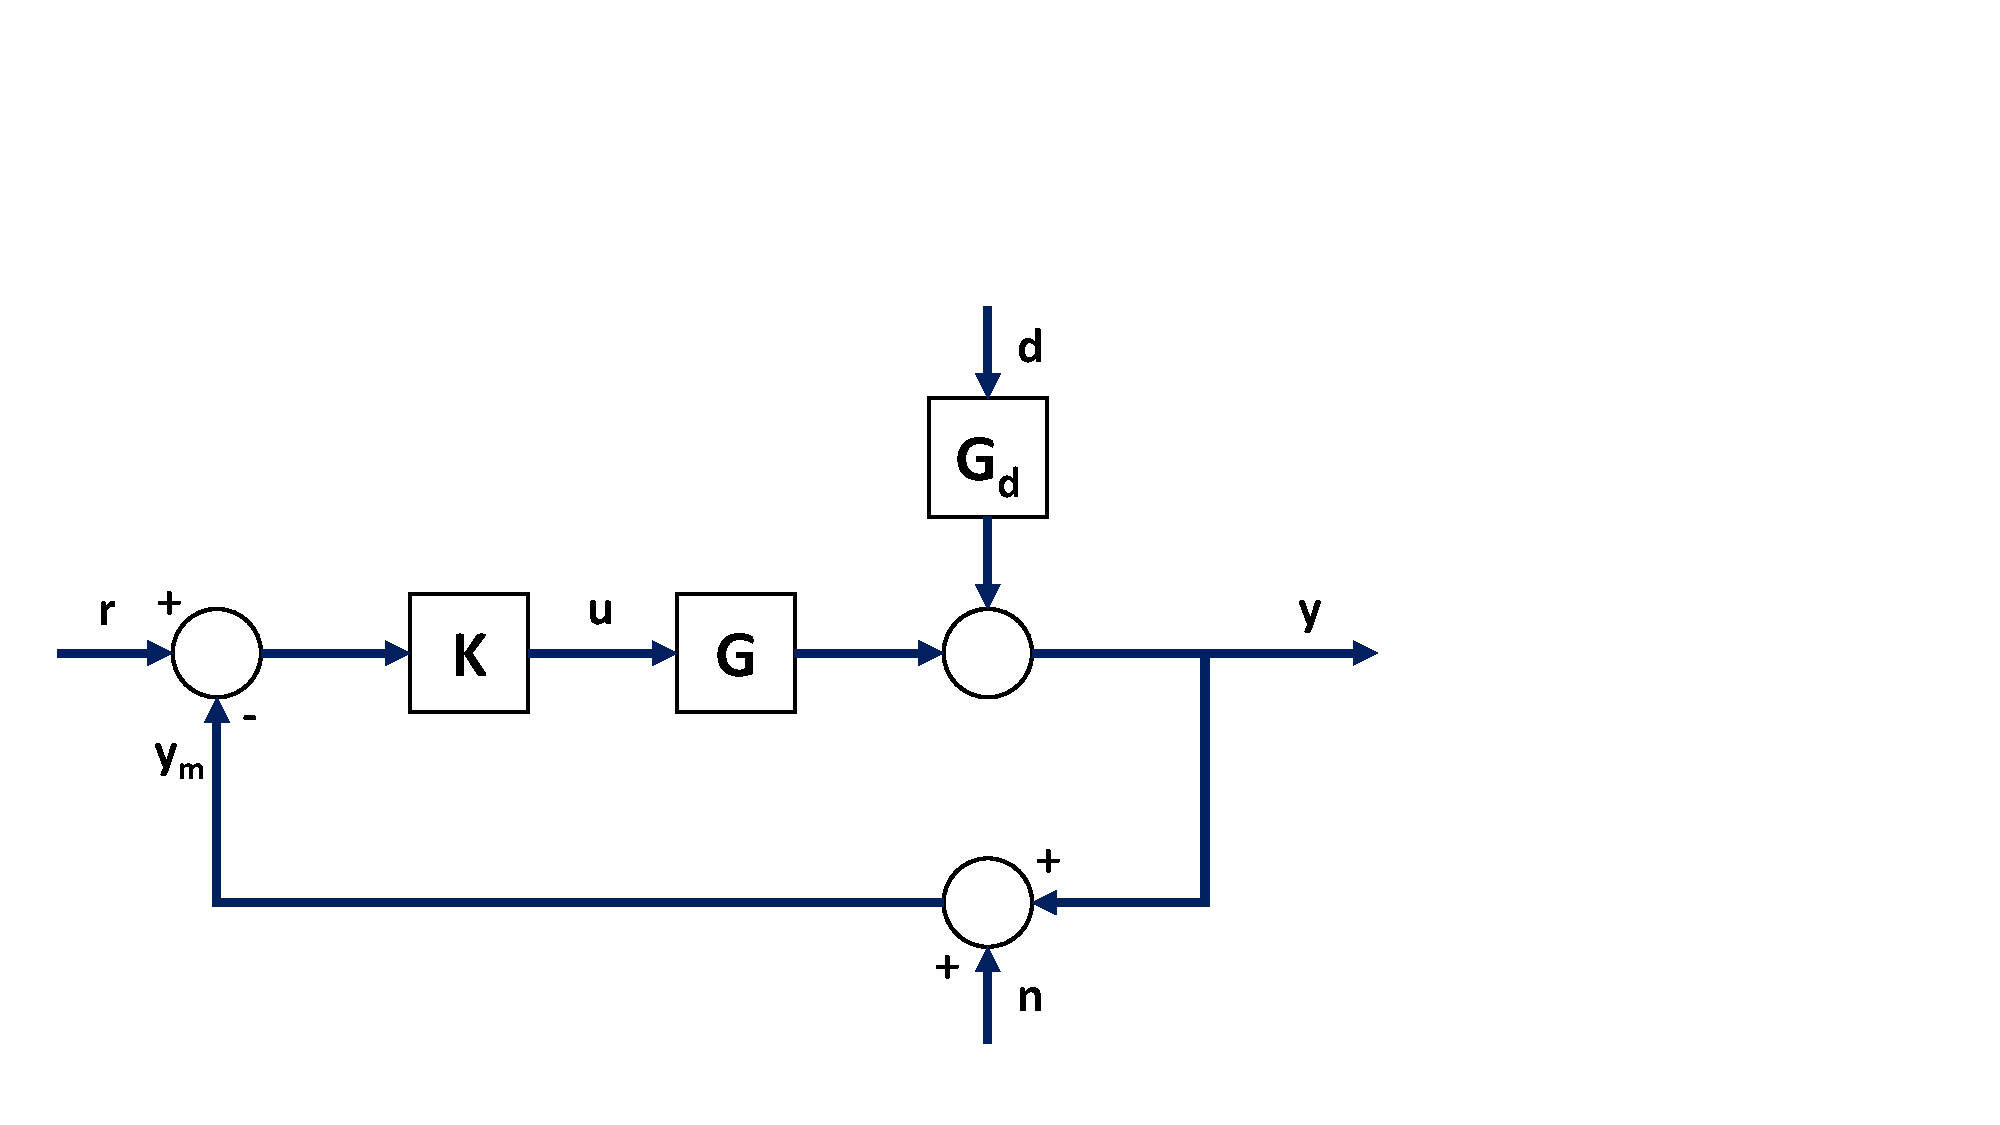
\includegraphics[trim = 20px 50px 300px 150px, clip, width=0.85\textwidth]{img/StandardRegelkreis_BSB}
\caption{Blockschaltbild des SISO-Standardregelkreises}
\end{figure}

Die Regelstrecke wird durch die Übertragungsfunktion $G$, der Regler von $K$ und die Stördynamik von $G_d$ beschrieben. Für die Analyse des geschlossenen Regelkreises ist der Einfluss der Stellgröße $r$, der Störgröße $d$ und des Messfehlers $n$ auf die Ausgangsgröße $y$ von Interesse, wofür sich 
\begin{equation}
u = K \cdot r = K \cdot ( r - n - y)
\end{equation}
\begin{equation}
\label{eq_standardregelkreis}
\begin{split}
y &= G_d \cdot d + G\cdot u =  G_d\cdot d + GK\cdot (r - n - y) \\
&= \underbrace{(1 + GK)^{-1}GK}_{= T} \cdot r + \underbrace{(1 + GK)^{-1}}_{\equiv S} G_d \cdot d - \underbrace{(1 + GK)^{-1}GK}_{= T} \cdot n \\
&= T\cdot r + S\cdot G_d \cdot d + T \cdot n
\end{split}
\end{equation}
ergibt, wobei $S$ als die Empfindlichkeitsfunktion und $T$ auf Grund von
\begin{equation}
\label{eq_empfindlichkeit}
T + S = 1
\end{equation}
als die komplementäre Empfindlichkeit bezeichnet wird. Aus Gleichung (\ref{eq_standardregelkreis}) ergeben sich bereits relevante Forderungen an den Regelkreis. Für gutes Führungsverhalten sollte 
\begin{equation}
y = r
\end{equation}
gelten, wofür $T$ möglichst nahe an $1$ liegen muss. Diese Forderung wird nach
\begin{equation}
T = \frac{GK}{1+GK}
\end{equation}
erfüllt, indem eine betragsmäßig möglichst große Reglerübertragungsfunktion $K$ gewählt wird. Im Umkehrschluss führen hohe Reglerwerte zu gutem Führungsverhalten des geschlossenen Regelkreises. Ebenso nimmt die Unempfindlichkeit gegenüber Störungen ab, da
\begin{equation}
S = (1+GK)^{-1}
\end{equation}
mit zunehmenden Reglerfaktoren kleiner wird. Allerdings wirkt der Messfehler $n$ proportional zu $T$ auf die Ausgangsgröße ein, weshalb mit zunehmender Reglerverstärkung Messfehler stärker ins Gewicht fallen. An dieser Stelle zeigt sich bereits ein grundsätzliches Problem des Reglerentwurfs, dass die Forderung nach Unempfindlichkeit gegenüber Störungen und Messfehlern nicht simultan erfüllt werden kann. Für die Lösung dieses Problems wird die Forderung auf ein relevantes Frequenzband beschränkt. Die Störungen bewegen sich für gewöhnlich in einem Frequenzbereich als Messfehler, weshalb die Forderungen an den Betrag von $S$ und $T$ frequenzabhängig formuliert werden sollten. Hierfür wird die Gewichtungsfunktion $w_P(s)$ zusammen mit der Forderung
\begin{equation}
{\lVert w_P(s)\cdot S(s) \rVert}_\infty < 1
\end{equation}
eingeführt, welche von dem Regler erfüllt werden muss \cite[S. 60 ff]{MFC}. Wird die Forderung eingehalten wird die nominelle Reglergüte erzielt. Allerdings gilt sowohl die Stabilitäts- als auch Güteaussage lediglich für das durch $G$ und $G_d$ spezifizierte Modelle. Bereits minimale Abweichungen, die sich nicht ausschließen lasse, führen dazu, dass die nominellen Stabilitäts- und Güteaussagen hinfällig sind. Aus diesem Grund wird der Begriff der robusten Stabilität und robusten Güte eingeführt, welche die nominelle Stabilität und Reglergüte auch bei spezifizierten Ungenauigkeiten garantieren.